% =======================================================================
\chapter{El repositorio}
\label{cap:repositorio}
% =======================================================================

El repositorio \texttt{Triple-Resolutive-Approach-repo} es el producto
central de este trabajo. No acompaña al paper: lo sostiene. Todas las cifras
del Capítulo~\ref{cap:paper} se derivan de artefactos que están versionados
en él, y cualquiera de ellas puede rastrearse hasta la corrida individual que
la produjo.

Este capítulo lo documenta desde la ingeniería de software: los principios
que guiaron su diseño, los requisitos que satisface, su arquitectura
—descrita con diagramas UML—, sus componentes, su uso y cómo extenderlo.

\section{Principios de diseño}

Tres decisiones estructurales explican la forma del repositorio:

\begin{description}
  \item[Interfaz uniforme.] Los quince módulos de Búsqueda Tabú exponen la
    misma función \texttt{solve()} y devuelven el mismo diccionario
    (Código~\ref{lst:interfaz}). El orquestador no contiene ninguna
    ramificación por problema.
  \item[Separación entre algoritmo e infraestructura.] Los módulos de
    \texttt{tabu\_search/} no saben nada de archivos, formatos ni métricas.
    Reciben un diccionario de datos y devuelven un diccionario de resultados.
    Toda la entrada/salida vive en \texttt{src/}.
  \item[Persistencia inmutable.] Cada corrida escribe su propio directorio con
    marca de tiempo. Nada se sobrescribe, de modo que re-ejecutar experimentos
    nunca destruye evidencia previa.
\end{description}

\section{Requisitos}
\label{sec:requisitos}

Los objetivos de la Sección~\ref{sec:objetivos} se traducen en los requisitos
de la Tabla~\ref{tab:requisitos}. Los funcionales describen qué debe hacer el
repositorio; los de calidad, cómo debe hacerlo~\cite{bass2012software}. La
última columna indica el componente que satisface cada uno.

\begin{table}[H]
\centering
\caption{Requisitos del repositorio y componente que los satisface}
\label{tab:requisitos}
\small
\begin{tabular}{lp{8.3cm}p{3.7cm}}
\toprule
\textbf{ID} & \textbf{Requisito} & \textbf{Componente} \\
\midrule
\multicolumn{3}{l}{\emph{Requisitos funcionales}} \\
RF1 & Ejecutar una combinación cualquiera de problema, instancia, nivel de
      TS y semilla desde la línea de comandos.
    & \texttt{main.py}, \texttt{runner.py} \\
RF2 & Ejecutar el diseño factorial completo (360 experimentos) con un solo
      comando.
    & \texttt{main.py} \\
RF3 & Persistir cada corrida con su valor, GAP, tiempo, historial de
      convergencia y solución.
    & \texttt{runner.py}, \texttt{output/} \\
RF4 & Consolidar las corridas en tablas con media y desviación estándar por
      instancia.
    & \texttt{reporter.py}, \texttt{results/} \\
RF5 & Verificar de forma independiente el óptimo de las instancias pequeñas.
    & \texttt{models/} \\
\midrule
\multicolumn{3}{l}{\emph{Requisitos de calidad}} \\
RC1 & Reproducibilidad: semillas fijas y dependencias con versión declarada.
    & \texttt{main.py}, \texttt{requirements.txt} \\
RC2 & Extensibilidad: agregar un problema o un nivel de TS sin modificar el
      orquestador.
    & interfaz \texttt{solve()} \\
RC3 & Trazabilidad: toda cifra publicada se rastrea hasta las corridas que
      la producen.
    & \texttt{output/}, \texttt{results/} \\
RC4 & Bajo acoplamiento: \texttt{solve()} recibe y devuelve diccionarios,
      sin leer ni escribir archivos.
    & \texttt{tabu\_search/} \\
\bottomrule
\end{tabular}
\end{table}

\section{Arquitectura de software}
\label{sec:arquitectura}

La arquitectura separa tres responsabilidades: la orquestación de los
experimentos, los algoritmos de Búsqueda Tabú y los servicios de
infraestructura (carga de instancias, métricas y reportes). Se documenta con
dos vistas UML~\cite{fowler2003uml}: una estructural y una de comportamiento.

\subsection{Vista estructural: diagrama de clases}

El repositorio se organiza en módulos de funciones y no en clases. Por eso,
en la Figura~\ref{fig:uml_clases_tesis} cada módulo se modela como una clase
con el estereotipo «módulo», cuyas operaciones son sus funciones públicas
(\texttt{+}) y privadas (\texttt{-}). La interfaz \texttt{SolverTS} no existe
como archivo: representa el contrato que cumplen los quince módulos de
\texttt{tabu\_search/}.

\begin{figure}[H]
  \centering
  \begin{tikzpicture}[
      clase/.style={draw, rectangle split, rectangle split parts=2,
                    align=left, font=\footnotesize\ttfamily, fill=gray!8,
                    inner sep=3pt, text width=6.7cm, anchor=north},
      dep/.style={->, >=stealth, dashed},
      real/.style={-{Triangle[open, length=6pt, width=7pt]}, dashed},
      rot/.style={font=\scriptsize\itshape, text=gray!90!black}]
    % Columna izquierda: orquestación y algoritmos
    \node[clase] (main) at (0,0)
      {\centering «módulo»\\\textbf{src/main.py}
       \nodepart{two}+ DEFAULT\_SEEDS: list[int]\\
       + main(): None\\
       + run\_all(seeds, verbose): None\\
       - \_list\_instances(problema): list[str]};
    \node[clase] (run) at (0,-3.3)
      {\centering «módulo»\\\textbf{src/runner.py}
       \nodepart{two}+ PROBLEMS, ALGORITHMS, EXTENSIONS\\
       + run\_experiment(problema, instancia,\\
       \ \ \ algoritmo, seed): dict\\
       - \_find\_instance\_file(...)\\
       - \_load\_solver(problema, algoritmo)\\
       - \_make\_output\_dir(...)};
    \node[clase] (ifz) at (0,-7.5)
      {\centering «interface»\\\textbf{SolverTS}
       \nodepart{two}+ solve(instance\_data, ..., seed): dict};
    \node[clase] (impl) at (0,-9.75)
      {\centering «módulo»\\\textbf{tabu\_search/\{problema\}/}
       \nodepart{two}ts\_basico.py\\ts\_intermedio.py\\ts\_avanzado.py};
    % Columna derecha: servicios de infraestructura
    \node[clase] (rep) at (7.7,0)
      {\centering «módulo»\\\textbf{src/reporter.py}
       \nodepart{two}+ generate\_report(verbose): None\\
       - \_load\_results(): list[dict]\\
       - \_aggregate\_results(records): dict\\
       - \_write\_consolidated(...)};
    \node[clase] (load) at (7.7,-3.3)
      {\centering «módulo»\\\textbf{src/loader.py}
       \nodepart{two}+ load\_instance(filepath): dict\\
       + load\_knapsack(filepath): dict\\
       + load\_tsp(filepath): dict\\
       + load\_vrp(filepath): dict\\
       + load\_flowshop(filepath): dict\\
       + load\_jobshop(filepath): dict};
    \node[clase] (met) at (7.7,-7.5)
      {\centering «módulo»\\\textbf{src/metrics.py}
       \nodepart{two}+ MINIMIZATION: dict[str, bool]\\
       + gap(value, bks, minimization): float\\
       + summarize(result, instance\_data,\\
       \ \ \ problema): dict};
    % Dependencias y realización
    \draw[dep] (main) -- (rep);
    \draw[dep] (main) -- (run);
    \draw[dep] (run) -- (load);
    \draw[dep] (run) -- node[right, rot]{importación dinámica} (ifz);
    \draw[dep] (run.south east) -- (met.north west);
    \draw[real] (impl) -- node[right, rot]{5 problemas $\times$ 3 niveles} (ifz);
  \end{tikzpicture}
  \caption{Diagrama de clases UML del repositorio. Las flechas punteadas
           indican dependencia; la flecha con triángulo hueco, la realización
           de la interfaz \texttt{solve()} por los quince módulos de TS.}
  \label{fig:uml_clases_tesis}
\end{figure}

El diagrama muestra tres propiedades de la arquitectura:

\begin{itemize}
  \item \texttt{runner.py} concentra las dependencias: usa
    \texttt{loader.py}, \texttt{metrics.py} y la interfaz \texttt{SolverTS},
    pero no conoce ningún módulo de TS en particular.
  \item \texttt{reporter.py} no depende de \texttt{runner.py}. Ambos se
    comunican a través de los archivos de \texttt{output/}; por eso el
    reporte puede regenerarse sin volver a ejecutar los experimentos.
  \item \texttt{loader.py} oculta los cinco formatos de instancia tras una
    única función, \texttt{load\_instance()}, que elige el \emph{parser}
    según la extensión del archivo.
\end{itemize}

\subsection{Patrones de diseño}

Dos decisiones de diseño explican el requisito de extensibilidad (RC2):

\begin{itemize}
  \item \textbf{Estrategia.} Los quince módulos de TS son estrategias
    intercambiables tras una misma firma, \texttt{solve()}, en el sentido del
    patrón \emph{Strategy}~\cite{gamma1994design}. El código cliente
    —\texttt{runner.py}— trata por igual a los tres niveles y a los cinco
    problemas.
  \item \textbf{Carga dinámica.} \texttt{runner.py} construye el nombre del
    módulo a partir del problema y del algoritmo —por ejemplo,
    \texttt{tabu\_search.\allowbreak tsp.\allowbreak ts\_basico}— y lo
    importa en tiempo de ejecución con \texttt{importlib}. Agregar una estrategia nueva
    exige crear un archivo y registrar su nombre, sin tocar el orquestador.
\end{itemize}

\subsection{Vista de comportamiento: diagrama de secuencia}

La Figura~\ref{fig:uml_secuencia} muestra la interacción entre los módulos
durante un experimento individual, es decir, una llamada a
\texttt{run\_experiment()}. El experimento completo repite esta secuencia
para cada una de las 360 combinaciones (Figura~\ref{fig:flujo_ejecucion}).

\begin{figure}[H]
  \centering
  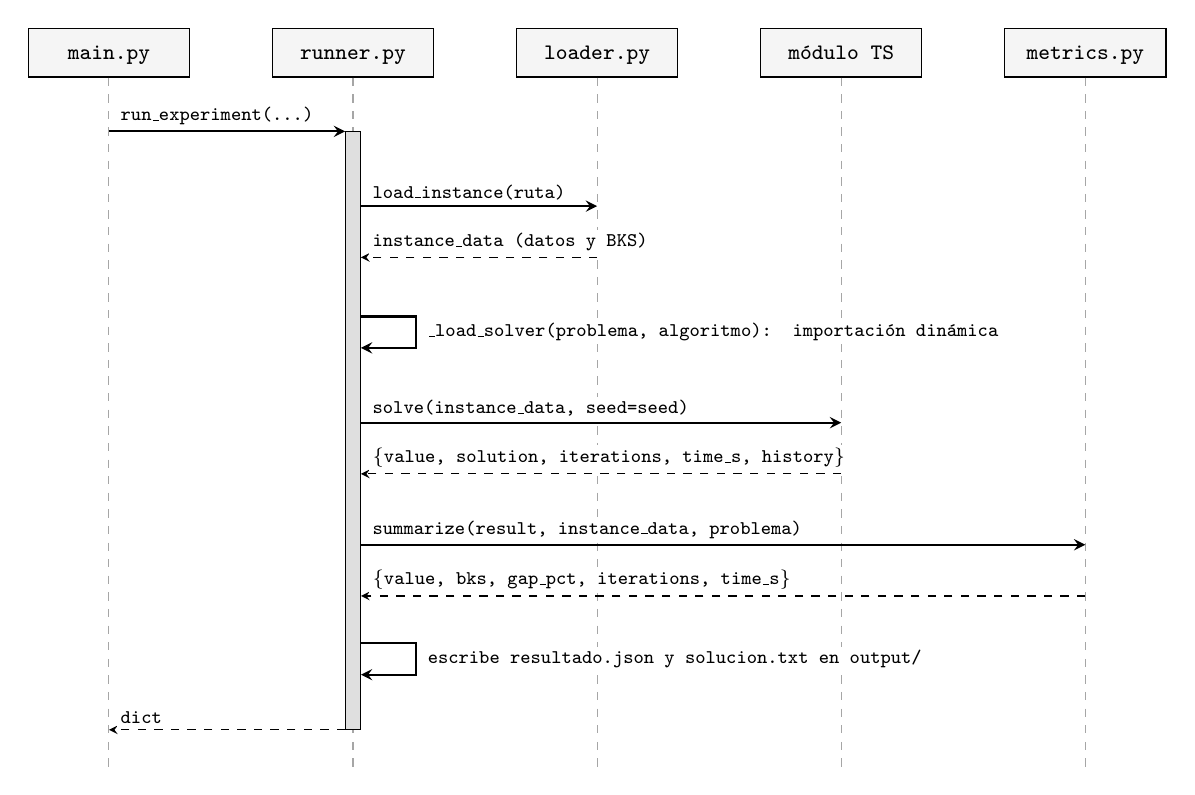
\begin{tikzpicture}[
      obj/.style={draw, fill=gray!8, font=\footnotesize\ttfamily,
                  minimum height=0.62cm, minimum width=2.05cm,
                  text height=1.6ex, text depth=0.4ex},
      vida/.style={dashed, gray!70},
      msg/.style={->, >=stealth, thick},
      ret/.style={->, >=stealth, dashed},
      etq/.style={font=\scriptsize\ttfamily, fill=white, inner sep=1.2pt}]
    % Participantes
    \node[obj] (m)  at (0,0)    {main.py};
    \node[obj] (r)  at (3.1,0)  {runner.py};
    \node[obj] (l)  at (6.2,0)  {loader.py};
    \node[obj] (t)  at (9.3,0)  {módulo TS};
    \node[obj] (me) at (12.4,0) {metrics.py};
    % Líneas de vida
    \foreach \o in {m,r,l,t,me}
      \draw[vida] (\o.south) -- ++(0,-8.75);
    % Activación de runner.py
    \draw[fill=gray!25] (3.0,-1.0) rectangle (3.2,-8.6);
    % 1. main -> runner
    \draw[msg] (0,-1.0) -- (3.0,-1.0);
    \node[etq, anchor=south west] at (0.1,-0.97) {run\_experiment(...)};
    % 2. runner -> loader
    \draw[msg] (3.2,-1.95) -- (6.2,-1.95);
    \node[etq, anchor=south west] at (3.3,-1.92) {load\_instance(ruta)};
    \draw[ret] (6.2,-2.6) -- (3.2,-2.6);
    \node[etq, anchor=south west] at (3.3,-2.57) {instance\_data (datos y BKS)};
    % 3. runner -> runner (importación dinámica)
    \draw[msg] (3.2,-3.35) -- ++(0.7,0) -- ++(0,-0.4) -- (3.2,-3.75);
    \node[etq, anchor=west] at (4.0,-3.55)
      {\_load\_solver(problema, algoritmo): importación dinámica};
    % 4. runner -> módulo TS
    \draw[msg] (3.2,-4.7) -- (9.3,-4.7);
    \node[etq, anchor=south west] at (3.3,-4.67) {solve(instance\_data, seed=seed)};
    \draw[ret] (9.3,-5.35) -- (3.2,-5.35);
    \node[etq, anchor=south west] at (3.3,-5.32)
      {\{value, solution, iterations, time\_s, history\}};
    % 5. runner -> metrics
    \draw[msg] (3.2,-6.25) -- (12.4,-6.25);
    \node[etq, anchor=south west] at (3.3,-6.22)
      {summarize(result, instance\_data, problema)};
    \draw[ret] (12.4,-6.9) -- (3.2,-6.9);
    \node[etq, anchor=south west] at (3.3,-6.87)
      {\{value, bks, gap\_pct, iterations, time\_s\}};
    % 6. runner -> runner (persistencia)
    \draw[msg] (3.2,-7.5) -- ++(0.7,0) -- ++(0,-0.4) -- (3.2,-7.9);
    \node[etq, anchor=west] at (4.0,-7.7)
      {escribe resultado.json y solucion.txt en output/};
    % 7. retorno a main
    \draw[ret] (3.0,-8.6) -- (0,-8.6);
    \node[etq, anchor=south west] at (0.1,-8.57) {dict};
  \end{tikzpicture}
  \caption{Diagrama de secuencia UML de un experimento individual. Las
           flechas continuas son llamadas; las punteadas, valores de retorno.}
  \label{fig:uml_secuencia}
\end{figure}

\section{Estructura de directorios}

\begin{figure}[H]
\footnotesize
\begin{verbatim}
Triple-Resolutive-Approach-repo/
|- instances/          Instancias benchmark (24 archivos)
|  |- knapsack/  .kp     tsp/  .tsp      vrp/  .vrp
|  `- flowshop/  .fsp    jobshop/ .jss
|- models/
|  |- ampl/            5 modelos AMPL de referencia exacta (.mod)
|  `- python_exact/    Solvers exactos: Knapsack DP, TSP Held-Karp, Flowshop
|- tabu_search/        15 modulos: 5 problemas x 3 niveles
|  |- knapsack/  ts_basico.py  ts_intermedio.py  ts_avanzado.py
|  `- tsp/  vrp/  flowshop/  jobshop/   (misma estructura)
|- src/
|  |- loader.py        Parsers de instancias y BKS
|  |- runner.py        Ejecutor de un experimento individual
|  |- metrics.py       Calculo de GAP y metricas
|  |- reporter.py      Consolidacion en CSV y tablas LaTeX
|  |- main.py          CLI principal
|  |- tables/          Tablas LaTeX por instancia (generadas)
|  `- utils/           Utilidades de exportacion de tablas
|- output/             Resultados crudos: un directorio por corrida
|- results/            CSVs consolidados por problema y global
|- notebooks/          5 cuadernos Jupyter de analisis
|- paper/              Paper IEEE en LaTeX (main.tex + secciones/ + figuras/)
|- EXPOTIC/            Afiche, articulo y presentacion del evento
|- TESIS/              Este documento
`- requirements.txt
\end{verbatim}
\caption{Estructura del repositorio.}
\label{fig:estructura_repo}
\end{figure}

\section{Componentes}

\subsection{\texttt{instances/} --- las entradas}

Contiene las 24 instancias benchmark en su formato original, con una
extensión por problema (\texttt{.kp}, \texttt{.tsp}, \texttt{.vrp},
\texttt{.fsp}, \texttt{.jss}). Los archivos no fueron modificados respecto a
la fuente, de modo que pueden contrastarse contra los repositorios públicos
originales.

\subsection{\texttt{tabu\_search/} --- los algoritmos}

El corazón del repositorio: quince módulos organizados en cinco carpetas, una
por problema, cada una con \texttt{ts\_basico.py}, \texttt{ts\_intermedio.py}
y \texttt{ts\_avanzado.py}. Cada módulo es autocontenido —implementa su propia
vecindad, su lista tabú y su heurística constructiva— y no importa nada de los
demás.

La progresión entre niveles se aprecia en el tamaño del código y en la
naturaleza de la memoria empleada: TS-Básico mantiene una \texttt{deque} de
tamaño fijo (Código~\ref{lst:basico}), mientras TS-Avanzado añade una matriz
de frecuencia, un parámetro de penalización adaptativo y un mecanismo de
perturbación estructural (Código~\ref{lst:avanzado}).

Cada módulo es además ejecutable directamente, lo que permite probar un
algoritmo sobre todas las instancias de su problema sin pasar por el
orquestador:

\begin{verbatim}
python tabu_search/tsp/ts_avanzado.py
\end{verbatim}

\subsection{\texttt{src/} --- la infraestructura}

Cinco módulos con responsabilidades disjuntas:

\begin{table}[H]
\centering
\caption{Módulos de infraestructura}
\label{tab:modulos_src}
\small
\begin{tabular}{llp{7cm}}
\toprule
\textbf{Módulo} & \textbf{Líneas} & \textbf{Responsabilidad} \\
\midrule
\texttt{loader.py}   & 392 & Parsers de los cinco formatos de instancia.
  Devuelve un diccionario con la matriz de datos y el BKS documentado. \\
\texttt{runner.py}   & 194 & Ejecuta un experimento individual: carga la
  instancia, importa dinámicamente el módulo de TS, invoca \texttt{solve()}
  y persiste el resultado. \\
\texttt{metrics.py}  &  68 & Cálculo del GAP respecto al BKS, con manejo del
  signo según sea problema de minimización o maximización
  (Código~\ref{lst:gap}). \\
\texttt{reporter.py} & 324 & Recorre \texttt{output/}, agrega por instancia
  y nivel, y genera los CSV de \texttt{results/} y las tablas LaTeX de
  \texttt{src/tables/}. \\
\texttt{main.py}     & 193 & Interfaz de línea de comandos y orquestación del
  producto cartesiano completo (Código~\ref{lst:orquestador}). \\
\bottomrule
\end{tabular}
\end{table}

La importación dinámica en \texttt{runner.py} es el detalle que hace
extensible el sistema: el nombre del módulo se construye a partir de los
argumentos \texttt{problema} y \texttt{algoritmo}, de modo que agregar un
módulo nuevo lo hace inmediatamente ejecutable sin tocar el orquestador.

\subsection{\texttt{models/} --- verificación independiente}

Dos vías de verificación del BKS:

\begin{itemize}
  \item \texttt{models/ampl/} --- cinco modelos exactos en AMPL
    (\texttt{knapsack.mod}, \texttt{tsp\_mtz.mod}, \texttt{cvrp.mod},
    \texttt{flowshop.mod}, \texttt{jobshop\_manne.mod}). Requieren licencia
    de AMPL.
  \item \texttt{models/python\_exact/} --- tres solvers exactos ejecutables
    sin dependencias comerciales: programación dinámica para Knapsack,
    Held-Karp para TSP y enumeración acotada para Flowshop. Permiten
    confirmar el óptimo en las instancias pequeñas.
\end{itemize}

\subsection{\texttt{output/} y \texttt{results/} --- la evidencia}

\texttt{output/} almacena los resultados crudos: un directorio por corrida,
nombrado \texttt{\{instancia\}\_\{algoritmo\}\_\{fecha\}/}, con dos archivos:

\begin{itemize}
  \item \texttt{resultado.json} --- valor obtenido, BKS, GAP, iteraciones,
    tiempo e historial completo de convergencia.
  \item \texttt{solucion.txt} --- la mejor solución encontrada en formato
    legible.
\end{itemize}

El historial de convergencia es lo que permite reconstruir las curvas del
paper sin re-ejecutar nada. \texttt{results/} contiene la vista agregada: un
CSV por problema más \texttt{tabla\_consolidada.csv}, con media y desviación
estándar del GAP y del tiempo sobre las cinco semillas.

Conviene precisar el alcance del material distribuido: el repositorio versiona
un \emph{subconjunto representativo} de las corridas crudas —del orden de 150
archivos— junto con los CSV consolidados completos, sustento de todas las cifras de este documento. El conjunto íntegro de las 360 corridas
ocupa aproximadamente \SI{40}{\mega\byte} en disco y se regenera con
\texttt{python src/main.py -{}-all -{}-multi-seed}. La decisión responde a
mantener el repositorio liviano sin perder la posibilidad de auditar los
resultados publicados.

\subsection{\texttt{notebooks/} --- el análisis}

Cinco cuadernos Jupyter, uno por problema, que reproducen el análisis visual
a partir de los CSV:

\begin{verbatim}
notebooks/analisis_knapsack.ipynb    notebooks/analisis_tsp.ipynb
notebooks/analisis_vrp.ipynb         notebooks/analisis_flowshop.ipynb
notebooks/analisis_jobshop.ipynb
\end{verbatim}

\subsection{\texttt{paper/}, \texttt{EXPOTIC/} y \texttt{TESIS/} --- las salidas}

Las tres formas de comunicar el trabajo: el artículo IEEE, el material
del evento EXPOTIC y este documento. Los tres se compilan desde el propio
repositorio y consumen las mismas figuras y tablas generadas por el código.

\section{Uso}

\subsection{Instalación}

\begin{verbatim}
git clone <url-del-repositorio>
cd Triple-Resolutive-Approach-repo
pip install -r requirements.txt
\end{verbatim}

\subsection{Comandos principales}

\begin{table}[H]
\centering
\caption{Comandos de uso frecuente}
\label{tab:comandos}
\small
\begin{tabular}{p{7.5cm}p{6cm}}
\toprule
\textbf{Comando} & \textbf{Efecto} \\
\midrule
\texttt{python src/main.py -{}-list} &
  Lista las instancias disponibles \\
\texttt{python src/main.py -{}-problema tsp -{}-instancia berlin52
  -{}-algoritmo ts\_basico} &
  Un experimento individual \\
\texttt{python src/main.py -{}-problema tsp -{}-all-instances
  -{}-all-algoritmos} &
  Todos los experimentos de un problema \\
\texttt{python src/main.py -{}-all} &
  72 experimentos, una semilla \\
\texttt{python src/main.py -{}-all -{}-multi-seed} &
  360 experimentos, cinco semillas (reproduce el paper) \\
\texttt{python src/main.py -{}-report} &
  Regenera los CSV consolidados \\
\texttt{python TESIS/generar\_figuras.py} &
  Regenera las figuras de este documento \\
\bottomrule
\end{tabular}
\end{table}

\section{Extensión}

La arquitectura fue pensada para crecer sin refactorizaciones. Los dos casos
de extensión previstos:

\subsection{Agregar un nivel de TS a un problema existente}

\begin{enumerate}
  \item Crear \texttt{tabu\_search/\{problema\}/ts\_\{nuevo\}.py} que exponga
    \texttt{solve(instance\_data, ..., seed) $\rightarrow$ dict} con las
    cinco claves de la interfaz.
  \item Añadir el nombre a la lista \texttt{ALGORITHMS} de
    \texttt{src/runner.py}.
\end{enumerate}

No se requiere ningún otro cambio: el orquestador, las métricas y el
generador de reportes lo incorporan automáticamente.

\subsection{Agregar un problema nuevo}

\begin{enumerate}
  \item Escribir el \emph{parser} en \texttt{src/loader.py} y registrar la
    extensión en \texttt{EXTENSIONS} de \texttt{src/runner.py}.
  \item Declarar en \texttt{MINIMIZATION} (\texttt{src/metrics.py}) si el
    problema es de minimización o maximización.
  \item Crear \texttt{tabu\_search/\{problema\}/} con los tres módulos.
  \item Depositar las instancias en \texttt{instances/\{problema\}/}.
\end{enumerate}

\section{Limitaciones conocidas}

Por transparencia, cuatro limitaciones del repositorio en su estado actual:

\begin{itemize}
  \item \textbf{Criterio de parada por iteraciones.} Los tiempos no son
    directamente comparables entre problemas ni entre niveles; una
    comparación estricta requeriría tiempo de CPU fijo.
  \item \textbf{Ejecución de un solo hilo.} No se aprovecha paralelismo, lo
    que limita el tamaño de las instancias abordables.
  \item \textbf{Sin pruebas automatizadas.} El repositorio no incluye una
    batería de pruebas unitarias. La verificación descansa en los modelos
    exactos de \texttt{models/} y en la reproducción de los resultados con
    semillas fijas.
  \item \textbf{Trazabilidad parcial en el repositorio.} Solo se versiona un
    subconjunto de las corridas crudas: el conjunto completo ocupa unos
    \SI{40}{\mega\byte} y se optó por mantener el repositorio liviano. Los CSV
    consolidados sí están completos, de modo que toda cifra publicada es
    verificable, pero auditar una corrida individual no incluida exige
    re-ejecutar el experimento.
\end{itemize}
